\chapter{Testowanie}
{\em \quad Analiza zgodności aplikacji PhotoLab z przyjętymi wymaganiami jest głównym tematem tego rozdziału. Tematyka testów znajduje się tutaj jedynie w celu zasygnalizowania, iż takowe testy się odbyły i stanowią bardzo ważna część procesu wdrożenia każdego nowego oprogramowania. Zostaną tutaj przytoczone jedynie podstawowe informacje o przeprowadzonych testach i~~ich parametrach, a także najciekawsze spostrzeżenia i wnioski z nich płynące. Zabraknie natomiast wnikliwego przedstawienia całego procesu przeprowadzenia testów, ich szczegółowych parametrów i wnikliwej analizy. Nie jest to przedmiotem tego rozdziału jak i całej dokumentacji.}



\section{Testy funkcjonalne}
\quad Są to testy czarnej skrzynki (\textit{ang. black box testing}). Istnieje bardzo wiele rodzajów tego typu testów, w tym konkretnym wypadku polegały one na przetestowaniu bardzo ważnego elementu jakim jest \textit{API} serwera. Przed rozpoczęciem testów konieczne było przygotowanie odpowiednich danych. Były nimi parametry wejściowe zapytań kierowanych do serwera, takie jak: adres zapytania, nagłówki czy różne parametry, a także oczekiwane wzorcowe dane wyjściowe, do których następnie zostały porównane wszystkie otrzymane wyniki. Zawierały one zarówno poprawne, jak i błędne parametry. Miało to na celu sprawdzenie nie tylko poprawności zwracanych rezultatów, ale także weryfikacji sposobu obsługi błędów w przypadku wystąpienia błędnych zapytań. \\
\\
Wszystkie testy zostały oparte o bardzo prosty, jednakże niezwykle użyteczny program \textit{\textbf{Postman}}, służący właśnie do tego typu zadań. Przykładowa prezentacja testu jednego z zapytań znajduje się na  rysunku \ref{fig:functional-tests}. Dotyczy ona sprawdzania metody kontrolera odpowiedzialnej za rejestrację użytkownika. W tym konkretnym przypadku użytkownik wprowadził poprawne dane, a konto o podanym adresie jeszcze nie istniało w systemie. Otrzymany rezultat był zgodny z oczekiwanym.\\
\\
Testy wykazały kilka niewielkich niezgodności w zwracanych przez system odpowiedziach. Szybka weryfikacja pozwoliła naprawić dostrzeżone błędy i tym sposobem uniknąć ich na serwerze produkcyjnym. Ostatecznie wszystkie przeprowadzone testy zakończyły się sukcesem.

 \begin{figure}[ht]
	\centering
	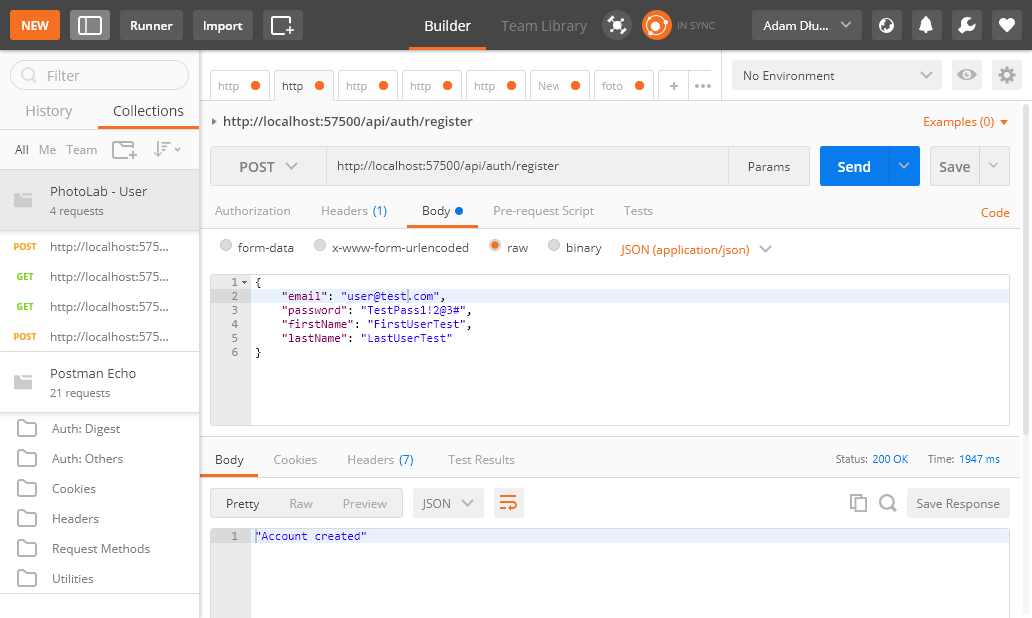
\includegraphics[width=1\linewidth]{graphics/chapter-5/functional-tests.png}
	\caption{Test funkcjonalny API z użyciem narzędzia PostMan}
	\label{fig:functional-tests}
\end{figure}


\newpage
\section{Testy użyteczności}
\quad W ramach testu przydatności i dostępności serwisu dla użytkowników zostały przeprowadzone testy użyteczności (\textit{ang. usability testing / user experience testing}). Podobnie do testów funkcjonalnych, również tego rodzaju testów istnieje wiele odmian i wariantów. Bardzo przykładem jest test typu \textit{eyetracking}, czyli badanie ruchu gałek ocznych, a zatem wędrówki wzroku użytkowników po serwisie www. Wynikiem takiego badania są tzw. \textit{head-mapy}, które pomagają określić np. na co na stronie największą uwagę zwracają klienci. Kolejnym interesującym testem jest nagrywanie zachowań osób odwiedzających witrynę. Specjalne narzędzie (np. aplikacja \textit{SmartLook}) wstrzyknięte w kod strony pozwala zapisywać każdy ruch użytkownika (ruchy myszki, wpisywane teksty, czy momenty zawahań i podejmowania decyzji). Powyższe sposoby nie zostały jednak wykorzystane do przeprowadzenia testów serwisu. Powodem ich dyskwalifikacji jest fakt, iż są to narzędzia wykorzystywane do badania stron, które zostały już opublikowane i korzysta z nich szerokie grono odbiorców. Wówczas analiza ich zachowań pozwala na modyfikację i podnoszenie jakości strony. \\
\\
W ramach badania użyteczności aplikacji \textit{PhotoLab} zdecydowano się na przeprowadzenie testów wykrywających obszary utrudniające realizację głównych założeń aplikacji oraz wpływających na negatywne odczucia użytkowników w trakcie korzystania ze strony.\\
Grupa testowa składała się z 6 osób - jest to liczba dość mała, jednak warunki projektowe nie pozwoliły przeprowadzić badań na większej grupie. Badani to 3 osoby w wieku 20-25 lat, 2~w przedziale 35-40 lat oraz jedna w wieku wyższym niż 55 lat - można również przyjąć, iż poziom znajomości obsługi komputerów był liniowo zależny do wieku użytkowników - osoba najstarsza posiadała najmniejszą wiedzę, najmłodsze - największą. Badani mieli do wykonania jeden zaplanowany scenariusz: wejście na stronę, zarejestrowanie nowego konta, zalogowanie użytkownika, zlecenie nowego zamówienia i ostatecznie z poziomu panelu użytkownika sprawdzenie statusu swojego zlecenia. Badanymi parametrami były między innymi: potrzebny czas na wykonanie scenariusza, popełnione błędy (podanie błędnych wartości, zagubienie na stronie, brak wiedzy o koniecznych do podjęcia kolejnych krokach, itp.), czy ogólne odczucia osób testujących.\\
\\
W ramach przedstawienia rezultatów przeprowadzonego testu można stwierdzić, iż ogólne odczucia badanych osób były bardzo pozytywne. Wszyscy użytkownicy samodzielnie ukończyli cały scenariusz w zbliżonym czasie (jedynie tester w wieku 55 lat rażąco odstawał od całego grona użytkowników - potrzebował dwukrotnie dłuższy czas niż najmłodsi, co jednak jest logiczne i nie jest specyfiką tylko aplikacji \textit{PhotoLab}). Przedstawiono także możliwości poprawy użyteczności głównie poprzez reorganizację kilku elementów strony. Zostały one uwzględnione i prawie wszystkie wdrożone (za wyjątkiem dwóch, które z technicznego punktu widzenia znacząco skomplikowałyby proces obsługi klienta).\\
\\
Test użyteczności zakończył się pozytywnym rezultatem. Wykazał kilka drobnych, wcześniej niedostrzeżonych elementów, które były stworzone nieoptymalnie dla potencjalnego klienta serwisu. Końcowe odczucia użytkowników były bardzo dobre, a sam system określony został jako przyjazny i przystępny dla każdego.

\section{Testy wydajnościowe}
\quad W ramach testów sprawdzających wydajność systemu zostały przeprowadzone 2 typy pomiarów: testy obciążenia (uwzględniające również test maksymalnego obciążenia) oraz testy wydajnościowe, które były zdecydowanie ważniejszym typem pomiarów. Testy uwzględniały naprzemienne wykonywanie dwóch scenariuszy biznesowych:
\begin{enumerate}
    \item Logowanie użytkownika i zlecania zamówienia.
    \item Logowanie administratora, przeglądanie wygenerowanych zleceń i ich edycja.
\end{enumerate}
Środowisko, które zostało wykorzystane do przeprowadzenia badań to w głównej mierze oprogramowanie \textit{Visual Studio} w wersji \textit{Enterprise 2017}, gdyż tylko taka wersja umożliwia wygenerowanie projektu typu \textit{Web Performance and Load Test Project}. Dodatkowo, aby nagrać scenariusz testowy zostało użyte oprogramowanie marki \textit{Telerik} - \textit{Fiddler}. Teoretycznie \textit{Visual Studio} zapewnia możliwość nagrywania scenariuszy poprzez wtyczkę do przeglądarki \textit{Internet Explorer 11}, jednakże nie spełniała ona swojej funkcji i została zastąpiona dodatkowym oprogramowaniem.\\
\\
Najważniejszym wynikiem przeprowadzonych testów było wykrycie błędu aplikacji będącej pod dużym obciążeniem. Serwis, z którego korzystało około 300 użytkowników jednocześnie rozpoczął generowanie błędów z serii \textit{500} - \textit{Internal Server Error}. Oznaczało to, iż stworzona aplikacja posiada wewnętrzny błąd, który ujawnia się dopiero przy dużym obciążeniu serwera (rys. \ref{fig:load-test-result-before-repair}).\\
\\
Analiza logów serwera wykazała, iż problem występuje w związku z połączeniem z bazą danych wychodzącym z kontrolera odpowiedzialnego za logowanie użytkownika. Polegał on na otwarciu zbyt wielu (ustawienia serwera ograniczały ilość do 100) aktywnych połączeń z bazą danych oczekujących asynchronicznie na jej odpowiedź. Pierwszym możliwym, chociaż niezalecanym sposobem uniknięcia tego błędu jest zwiększenie domyślnego parametru otwartych połączeń z bazą danych (\textit{ang. max pool size}). Nie jest to jednak rozwiązanie dobre, gdyż jak wynika z dokumentacji tej technologii, domyślna liczba w zupełności wystarcza nawet dużym i~obciążonym systemom. Należało wiec poszukać błędu w samym kodzie metody \textit{login()}. Jak się ostatecznie okazało, faktycznie występowało tam redundantne odpytywanie bazy danych o~dane użytkownika. Wynikało to z faktu, iż metoda ta zawierała zarówno kod biblioteki \textit{ASP.NET Identity}, a także generator kluczy \textit{JWT} i wystąpił tutaj typowy błąd programistyczny niepoprawnie stworzonej obsługi zapytania. Po dokonaniu odpowiednich modyfikacji i~ponownym przetestowaniu aplikacji okazało się, iż problem został wyeliminowany, a~poza uniknięciem generowanie błędów stanowczo zmalało również obciążenie procesora (rys. \ref{fig:load-test-result-after-repair}).
 \begin{figure}[ht]
	\centering
	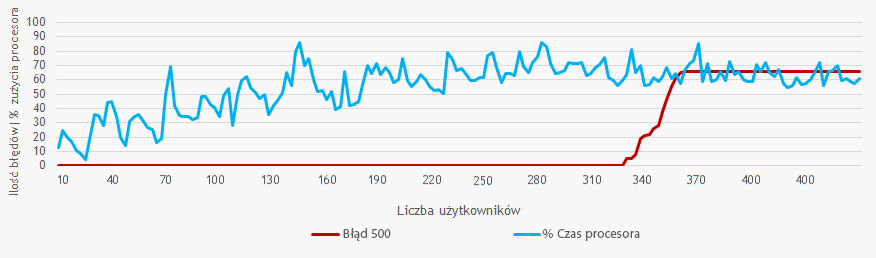
\includegraphics[width=1\linewidth]{graphics/chapter-5/load-test-result-before-repair.png}
	\caption{Test obciążenia serwera po wykryciu błędów typu 500}
	\label{fig:load-test-result-before-repair}
\end{figure}
 \begin{figure}[ht]
	\centering
	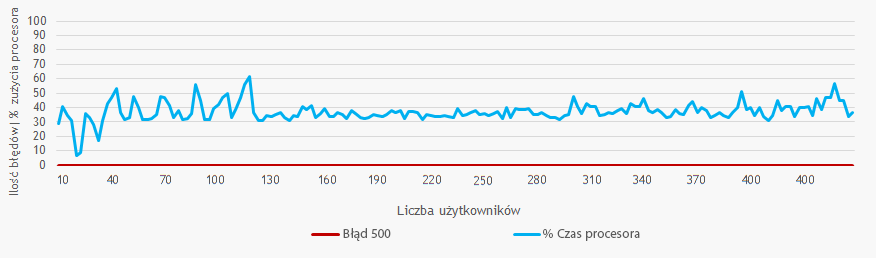
\includegraphics[width=1\linewidth]{graphics/chapter-5/load-test-result-after-repair.png}
	\caption{Test obciążenia serwera po eliminacji błędów typu 500}
	\label{fig:load-test-result-after-repair}
\end{figure}


\noindent Udało się również przeprowadzić testy wydajności niektórych, najważniejszych, zapytań serwera takich jak: \textit{getOrders()}, \textit{getUsers()}, \textit{submitOrder()}. Wykazały one, iż zapytania obsługiwane są w zadowalającym czasie. Jedynym \textit{requestem}, który znacznie odbiegał czasem odpowiedzi od pozostałych było zapytanie z prośbą o zwrócenie wszystkich znajdujących się w systemie zamówień. Udało się je jednak zoptymalizować poprzez skonkretyzowanie zwracanych informacji i znaczne zmniejszenie ich liczby, która była zbędna i nie wykorzystywana przez aplikację kliencką.
\newpage

\vspace*{0.01\baselineskip}

\section{Zgodność z wymaganiami}
\quad W momencie, gdy aplikacja została już w pełni zbudowana oraz przetestowana można określić jej poziom zgodność z założonymi w pierwszym etapie realizacji wymaganiami.\\
\\
Rozpoczynając podsumowanie od założeń technicznych należy stwierdzić, iż wykorzystanie wszystkich planowanych technologii, a także architektury trójwarstwowej zostało spełnione. W trakcie realizacji projektu nie napotkano na problemy, które mogłyby spowodować konieczność zmiany podejścia do architektury lub technologii. Jedynym odstępstwem jest zaimplementowanie serwera aplikacji w technologii \textit{.Net Core} w wersji \textit{2.0}, która jest wersją nowszą od planowej \textit{1.1}, a która w momencie projektowania była najnowszą wersją (dlatego też wersja \textit{2.0} nie została wówczas uwzględniona).\\
\\
Mówiąc o kompletności spełnienia założeń funkcjonalnych również można powiedzieć o~pełnym sukcesie. Udało się zaimplementować wszystkie funkcjonalności podstawowe, a~także planowane jako opcjonalne - funkcjonalności dodatkowe. Mimo ograniczonych ram czasowych na realizację projektu, szybki postęp prac pozwolił skupić się na implementacji wszystkich zakładanych funkcji systemu.\\
\\
Ostatnim, a zarazem najważniejszym wymogiem projektu było spełnienie jego czterech podstawowych celów. Były to: prostota użytkowania, przystępny koszt wdrożenia i utrzymania, bezpieczeństwo danych i transakcji oraz pokrycie wszystkich funkcjonalności oferowanych przez laboratorium w aplikacji internetowej. \\
\\
Analizując kolejno każdy z wymogów można stwierdzić iż:
\begin{enumerate}
    \item Przeprowadzone testy użyteczności wykazały łatwą dostępność, prostotę interfejsu i pozytywne wrażenia estetyczne budowanego serwisu podtrzymując przy tym tezę, iż użytkowanie systemu jest bezproblemowe.
    \item Jednoosobowy zespół projektowy, krótki okres wdrożenia (około 2 miesiące) i bardzo tani lub wręcz darmowy hosting przemawiają za tym, iż koszta poniesione na realizację autentycznego projektu nie mogłyby być wygórowane.
    \item Zaimplementowanie biblioteki \textit{ASP.NET Identity} oraz standardu \textit{JWT Token}, a także przeprowadzenie testów zarówno funkcjonalnych jak i wydajnościowych powoduje, iż aplikacja posiada wysoki (jak na możliwości projektowe i nakład środków) poziom zabezpieczeń.
    \item Ponieważ cały możliwy zakres oferty laboratorium został ustalony i spisany w formie funkcjonalności podstawowych i rozszerzonych, które z kolei zostały kompletnie zaimplementowane należy uznać, iż projekt spełnia również założenia ostatniego celu - pokrycia oferty zakładu w formie stacjonarnej, funkcjonalnościami serwisu online.
\end{enumerate}

